\documentclass[12pt]{article}
\usepackage[english]{babel}
\usepackage[utf8]{inputenc} % Permite el uso de caracteres del Español
\usepackage[T1]{fontenc}
\usepackage{graphicx}
\usepackage{amsmath}
\usepackage{wrapfig}
\usepackage{enumerate}
\usepackage[top=1in, bottom=1.25in, left=1.1in, right=1.1in]{geometry}
\usepackage[dvipsnames]{xcolor}
\usepackage{subcaption}

\begin{document}

\begin{titlepage}

\newcommand{\HRule}{\rule{\linewidth}{0.5mm}} % Define un comando para las lineas horizontales

\center 
%----------------------------------------------------------------------------------------
%	Cabezera
%----------------------------------------------------------------------------------------

\textsc{\LARGE Universidad de Sonora}\\[1.5cm]
\textsc{\Large Licenciatura en Física}\\[0.5cm]
\textsc{\large Física Computacional I}\\[0.5cm]

%----------------------------------------------------------------------------------------
%	Titulo
%----------------------------------------------------------------------------------------

\HRule \\[0.4cm]
{\huge \bfseries Evaluación I}\\[0.4cm] % Title of your document
\HRule \\[1.5cm]
 
%----------------------------------------------------------------------------------------
%	Autor
%----------------------------------------------------------------------------------------

\begin{minipage}{0.4\textwidth}
\begin{flushleft} \large
\emph{Alumno:}\\
José Gabriel Navarro I.
\end{flushleft}
\end{minipage}
~
\begin{minipage}{0.4\textwidth}
\begin{flushright} \large
\emph{Profesor:} \\
Carlos Lizarraga Celaya
\end{flushright}
\end{minipage}\\[2cm]


%----------------------------------------------------------------------------------------
%	Fecha
%----------------------------------------------------------------------------------------
08 de Marzo de 2018

%----------------------------------------------------------------------------------------
%	Escudo
%----------------------------------------------------------------------------------------


\includegraphics[width=0.4\textwidth]{logo.png}\\
 
%----------------------------------------------------------------------------------------

\vfill % Llena el espacio de la pagina en blanco

\end{titlepage}

En el presente reporte se habla acerca de la primera evaluación de la materia Física Computacional I, que abarca el tema de tratamiento de archivos y su análisis con el uso de Python y las librerías pandas y matplotlib.  \\

Los datos utilizados para esta evaluación fueron datos reales tomados de una estación de monitoreo de variables atmosféricas como lo son el CO2, radiación solar, nivel de agua y salinidad en el Manglar El Sargento, en una bahía en la costa frente a la parte norte de la Isla Tiburón. En este caso, se presentan el análisis de estos datos, haciendo énfasis en la temperatura del agua, nivel del mar y la salinidad. El nivel del mar sirve como referencia para ubicar la altitud de las localidades y accidentes geográficos, y la salinidad como su nombre lo indica, es la cantidad de sal disuelta en un cuerpo de agua. 

\section{Análisis de datos}
Primeramente se descargaron los datos correspondientes a la práctica en la página del curso. Una vez realizado esto, se observaron los contenidos del archivo para saber que datos eliminar. Los archivos presentaban distintas columnas, y distintas horas, uno presentaba temperatura con la salinidad mientras que otro presentaba el nivel del mar con su temperatura y otros datos. \\

En este caso, se elimino el desfase que había con los tiempos, uno siendo a las 12:45 y otro a las 11:15. Esto no se realizo con emacs. Se realizo utilizando los comandos drop y skiprow al leer el archivo en Jupyter Notebook. También, como se pasaron los primeros renglones, se le dieron un nuevo nombre a las columnas. \\

\begin{figure}[h]
    \centering
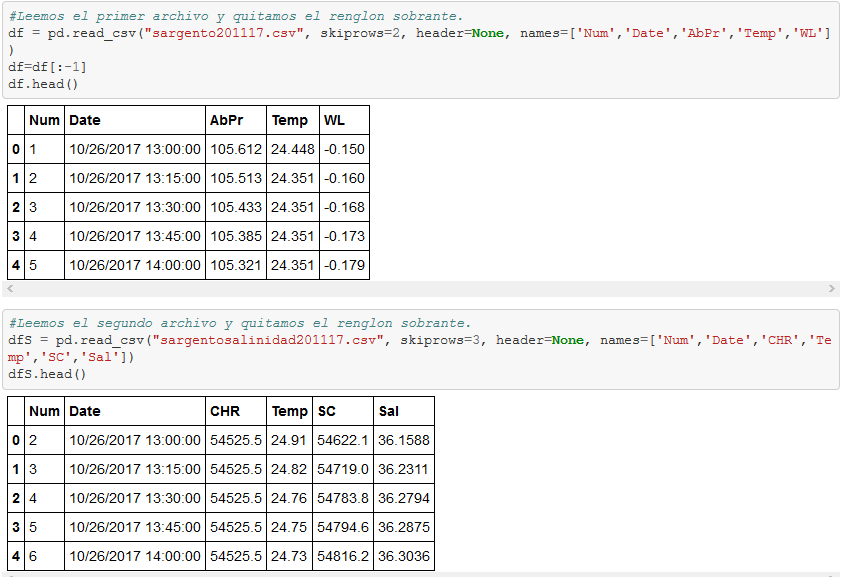
\includegraphics[width=5in]{Datos.png}
\end{figure}

Una vez echo esto, cambiamos el tipo de dato de la columna de fecha para ambos data frames, ya que estas fueron leídas como objetos. Esto se hizo mediante el uso de la librería datetime:

\begin{figure}[h]
    \centering
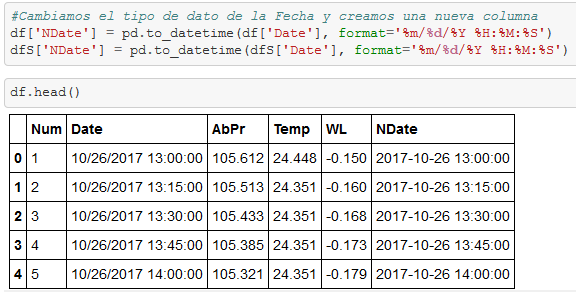
\includegraphics[width=4in]{date.png}
\end{figure}

Con esto, ya es posible realizar las graficas que se requieren para la evaluación. Sin embargo, para mayor facilidad al graficar algunas de ellas, se crearon nuevos dataframes, en donde solo se contienen las columnas necesarias para su graficación, esto se hizo mediante la creación de un nuevo dataframe seleccionando las columnas requeridas de los archivos:

\begin{figure}[h]
    \centering
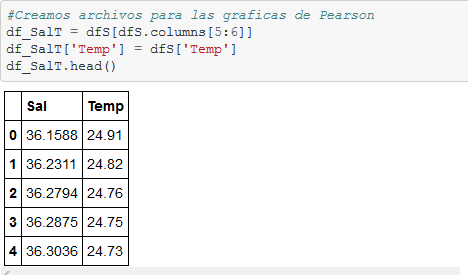
\includegraphics[width=3in]{Nuevodf.png}
\end{figure}

De esta manera, se procedió a realizar las graficas correspondientes a la evaluación. 

\section{Análisis de resultados}
En esta sección, se presentan las distintas graficas con su interpretación respectiva que se pedía en la evaluación. \\

\noindent\textbf {Con la ayuda de la biblioteca Seaborn,  por favor crea un gráfica de caja (boxplot) para visualizar la variabilidad de los datos de Febrero: } \\

\noindent\textbf {a) Nivel de mar (metros)} \\ \\

\begin{figure}[h]
    \centering
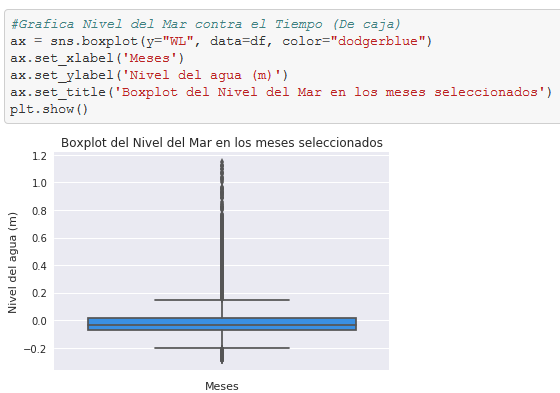
\includegraphics[width=4.5in]{Caja1.png}
\end{figure}

Para realizar esta gráfica, solamente se coloco en el eje de las 'y' el dato a analizar, sin separarlo en los distintos meses para estudiarlo de una mejor manera. En esta gráfica podemos observar como existe muchos puntos sesgados, es decir, fuera de la caja, la media y cuartiles están muy cerca de 0, causando que los datos mayores a estos sean sesgados (que son la mayoria). Esto puede observarse también en la descripción de los datos:

\begin{figure}[h]
    \centering
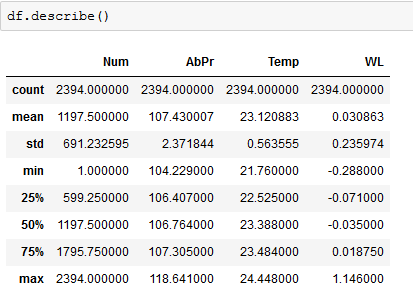
\includegraphics[width=4in]{dfdescribe.png}
\end{figure}
 
 En donde la mediana esta en 0.030 para WL (Water Level), y lo cuartiles es -0.07 y 0.018. Por lo cual muchos de los datos estan sesgados. \\
 
\noindent\textbf { b) Salinidad (Partes por mil - ppt)} \\

\begin{figure}[h]
    \centering
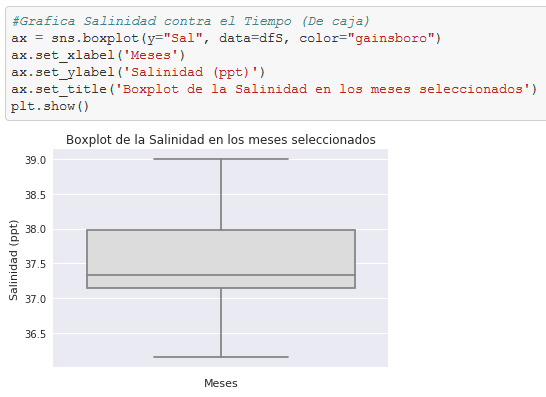
\includegraphics[width=4.5in]{Caja2.png}
\end{figure}

Para graficar esta y el resto de las graficas de caja se realizo el mismo proceso que en la gráfica anterior, colocando el dato a estudiar en el eje y. En el caso de la salinidad, podemos observar que ninguno de los datos están sesgados:

\begin{figure}[h]
    \centering
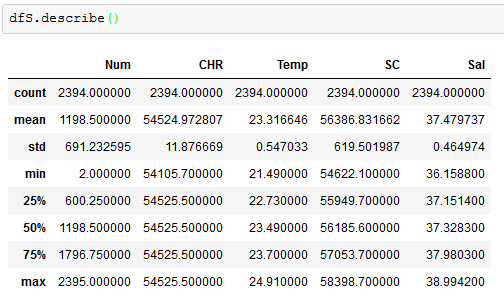
\includegraphics[width=4.5in]{dfSdescribe.png}
\end{figure}

Podemos observar como el valor máximo y mínimo, (36.15 y 38.99 respectivamente), están incluidos dentro de la línea de la caja.  \\

\noindent\textbf {c) Temperatura de Agua (ºC)}
\begin{figure}[h]
    \centering
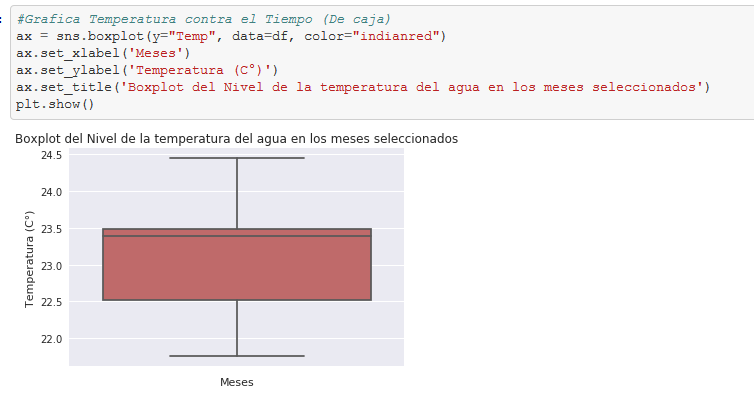
\includegraphics[width=5in]{Caja3.png}
\end{figure}

De igual manera que la gráfica anterior, podemos observar como ninguno de sus datos están sesgados, pero su media esta mas cargada al tercer cuartil. Esto se puede observar con la tabla de la función describe: \\ \\ \\

\begin{figure}[h]
    \centering
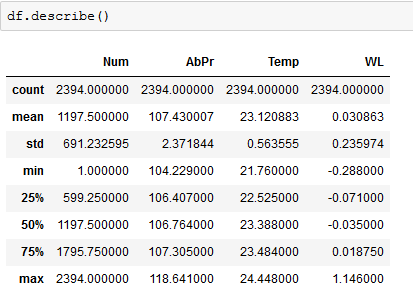
\includegraphics[width=4in]{dfdescribe.png}
\end{figure}

\noindent\textbf {De nuevo con la ayuda de Seaborn, también explora si hay una correlación de Pearson entre cada pareja de variables: } \\

\noindent\textbf {a) Nivel de mar-Salinidad} \\

\begin{figure}[h]
    \centering
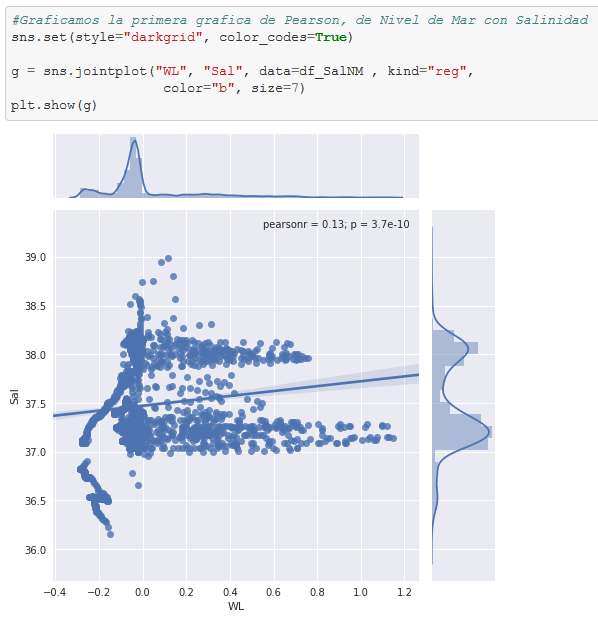
\includegraphics[width=3.45in]{Pearson1.png}
\end{figure}

Esta gráfica se realizó como se hizo anteriormente en clases, utilizando la libreria seaborn, indicando las dos variables a comparar, en este caso Nivel de mar y Salinidad. Es en estas graficas que se utiliza los nuevos dataframes creados anteriormente. En ella podemos observar un coeficiente de relación lineal de 0.13, con un factor de "no-relación" muy pequeño, lo cual nos dice que si hay poco de relación lineal entre estas dos variables. \\ 

\noindent\textbf {b) Nivel de mar-Temperatura del agua} \\
\begin{figure}[h!]
    \centering
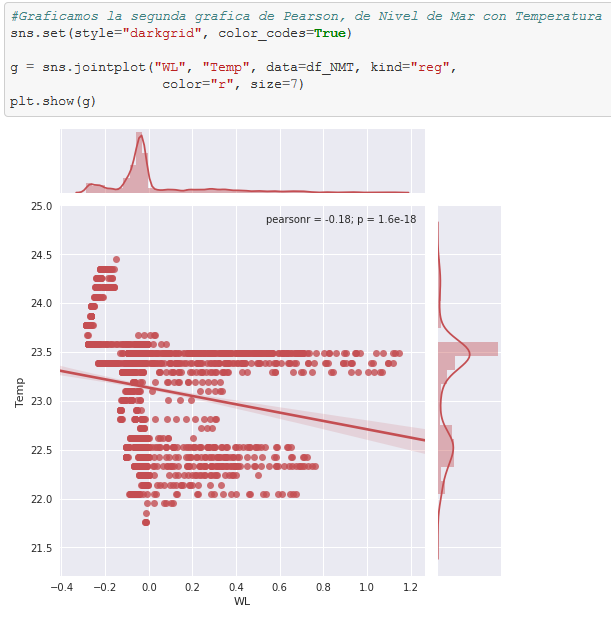
\includegraphics[width=3.45in]{Pearson2.png}
\end{figure}

De igual manera, esta gráfica se realizo utilizando la librería seaborn, indicando los datos a usar, y de donde extraemos esta información. Esta vez se relaciona el nivel de mar con la temperatura del agua, que, como podemos observar, esta gráfica tiene una relación parecida a la anterior, con un valor de 0.13, pero esta vez negativo, indicando una recta hacia abajo. \\

\noindent\textbf {c) Salinidad-Temperatura del agua} \\ \\
Por último, se muestra la gráfica que relaciona a la salinidad y la temperatura del agua, donde como se puede observar tienen un coeficiente de relación de -1. Eso indica que la relación entre temperatura y salinidad es casi seguro. \\

Al revisar estos datos y compararlos con los otros datos obtenidos de temperatura, se llego auna grafica muy parecida, con unos puntos mas dispersos pero con un coeficiente igual, de -1. \\ \\

\begin{figure}[h]
    \centering
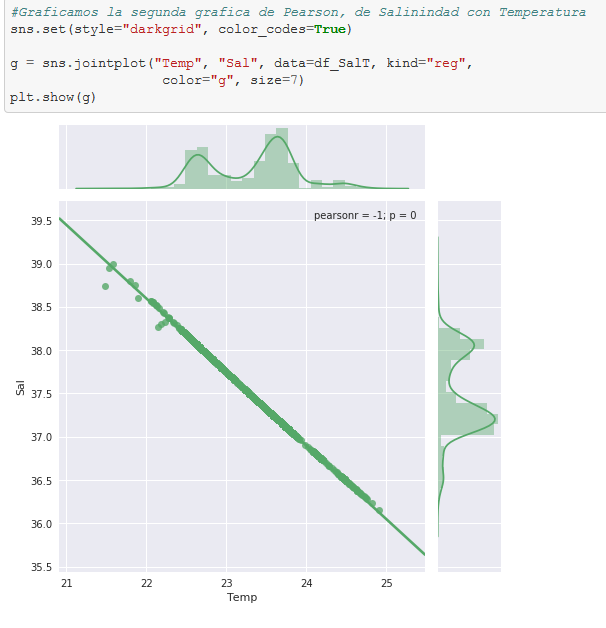
\includegraphics[width=3.45in]{Pearson3.png}
\end{figure}

\noindent\textbf {Con la ayuda de Matplotlib, realize ahora 3 gráficas independientes de las variables: } \\

\noindent\textbf {a) Nivel del mar} \\
\begin{figure}[h!]
    \centering
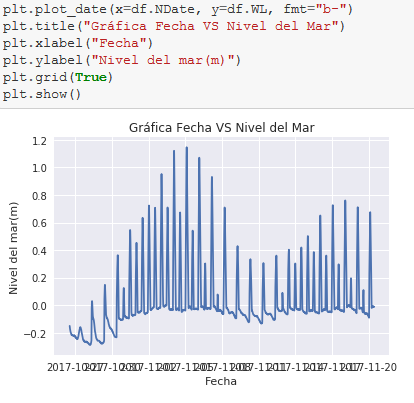
\includegraphics[width=3.8in]{GrafF1.png}
\end{figure}

Esta gráfica fueron de las primeras que se realizaron al inicio del semestre, en donde se indica el tipo de gráfica que es (date), seguido por los datos a graficar (en este caso el nivel del mar), en donde fmt permite cambiar el color de la gráfica. Como se puede observar, los picos mas altos están entre el día 5 de noviembre.  \\

\noindent\textbf {b) Salinidad} \\ \\
En esta gráfica y la siguiente se realizo el mismo proceso que la anterior, seleccionando los datos y poniéndolos en contra de las fechas. Esta es la salinidad contra el tiempo:

\begin{figure}[h!]
    \centering
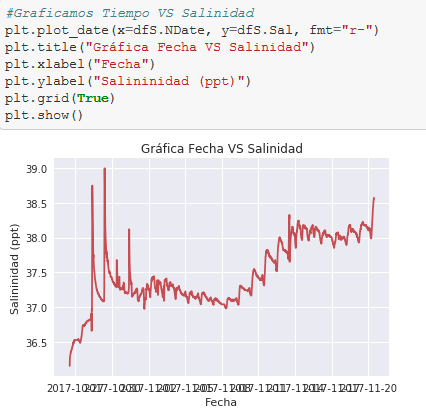
\includegraphics[width=3.8in]{GrafF2.png}
\end{figure}

Como podemos notar, en los primeros datos la cantidad era la menor de todos los registros, pero es en estos mismos días que aumenta y toma su valor máximo. \\

\noindent\textbf {c) Temperatura del agua} \\ \\
Por último se presenta la gráfica de la Temperatura con respecto el tiempo, en donde como podemos observar esta baja conforme el tiempo avanza. \\

Los datos están tomados en Octubre y en Noviembre, y como en Noviembre hace mas frío que Octubre, esto puede explicar el hecho de porque al avanzar el tiempo la temperatura del agua es cada vez menor. Sin embargo, esta temperatura no es exactamente muy grande, si observamos las tablas del comando describe, podemos ver como la mínima temperatura registrada es de 21.76$^{\circ}$C y la máxima es de 24.44$^{\circ}$C. \\

\begin{figure}[h!]
    \centering
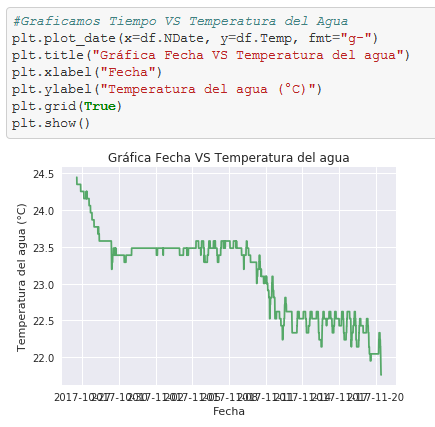
\includegraphics[width=3.8in]{GrafF3.png}
\end{figure}

\noindent\textbf {Enseguida, de igual forma, produce gráficas superpuestas con doble eje vertical (izquierda, derecha):} \\

\noindent\textbf {a) Nivel de mar y Salinidad}
\begin{figure}[h!]
    \centering
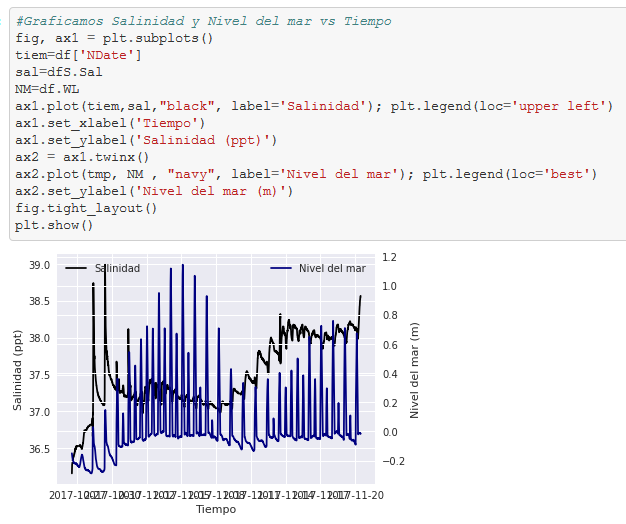
\includegraphics[width=4.3in]{SP1.png}
\end{figure}

En esta gráfica se utilizo un nuevo concepto de graficas que no se había visto en clases. Se utilizan los "subplots", que estos pueden ser colocados posteriormente en una figura, o "fig". De esta manera es posible graficar dos lineas con datos distintos en y, pero el mismo eje x. Solo es cuestión de definir de donde se tomaran los datos y definir ambas lineas que se van a graficar. \\

Parece que al analizar la gráfica, podemos observar que al bajar mas el nivel del mar la salinidad aumenta, esto se puede ver mas claro en los primeras fechas. Esto se puede observar mejor en el siguiente paso de la evaluación. \\

\noindent\textbf {b) Nivel de mar y Temperatura.} \\ \\
Esta gráfica se realizo de la misma manera que la anterior, tomando esta vez los datos de Fecha, Temperatura del agua y el nivel del mar. \\

En este caso, no se puede apreciar exactamente una relación clara entre estas dos variables, pero si tomamos un rango de días, podamos observar mejor estos fenómenos. \\ \\ \\ \\ \\ \\ \\ \\ \\ \\ \\ \\

\begin{figure}[h!]
    \centering
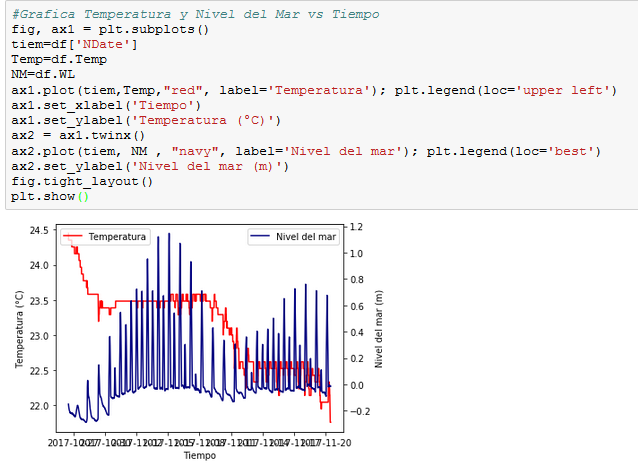
\includegraphics[width=6in]{SP2.png}
\end{figure}

\noindent\textbf {Con ayuda de la función xlim de pyplot, analiza las gráficas del punto anterior para 5 días y trata de explicar si hay o no una clara manifestación de dependencia de Salinidad y Nivel de mar o de Nivel de Mar y Temperatura del agua. } \\

\noindent\textbf {a) Nivel de mar y Salinidad} 

\begin{figure}[h!]
    \centering
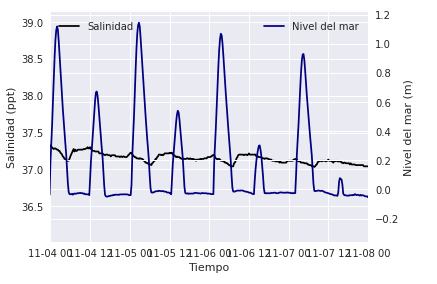
\includegraphics[width=4.3in]{SP1lim.png}
\end{figure}

Para realizar esta gráfica se tomo la gráfica anterior correspondiente a estos datos y solamente se modificaron los limites del eje x, siendo este el código: \textbf{plt.xlim(("2017-11-4 00:00:00","2017-11-8 00:00:00"))}, en donde se tomo del día 4 de Noviembre hasta el 8. \\

En este caso podemos observar como al tener niveles bajos de salinidad el nivel del mar tiene picos, lo que significa que si existe una relación entre estas dos variables. \\

\noindent\textbf {b) Nivel de mar y Temperatura} \\ \\
Al igual que la gráfica anterior, se tomo el mismo intervalo de 4 de noviembre a 8 de noviembre, tomando un intervalo de 5 días. Solamente se tomo la gráfica anterior y se modificaron los limites. \\

En este intervalo no se puede observar una relación exacta, pero si podemos notar que en algunos de los picos del Nivel del Mar, la Temperatura baja un poco. Por tanto la relación no es tan clara, pero si están relacionadas en alguna manera estas dos variables. 

\begin{figure}[h!]
    \centering
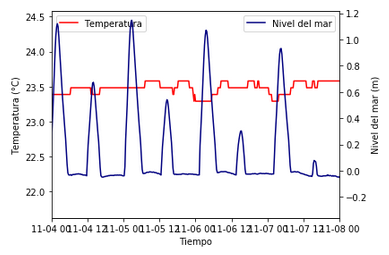
\includegraphics[width=5in]{SP2lim.png}
\end{figure}
\vfill

\section{Conclusiones}
Al terminar esta evaluación me di cuenta que el proceso de limpieza puede facilitarse mas al combinarse tanto las herramientas de pandas con Python y emacs, observando así los datos con ambos programas para ver de que manera es mas eficiente limpiarlos. \\

Al realizar esta evaluación, también me di cuenta de que aun hay muchas cosas mas por explorar en muchas de las librerías que utilizamos, sobre todo en matplotlib y seaborn, donde las graficas que se pueden realizar con ellas y la información que podemos concluir de ellas nos puede ayudar mucho en nuestra carrera. \\

Por último, me pareció muy interesante el tema que se trato en esta evaluación y la información que se encontró mediante el uso de las gráficas solicitadas como lo es la correlación entre distintas variables. Sin embargo, el tiempo que oficialmente se dio para realizar este examen se me hizo muy poco, la práctica era muy extensa para el tiempo. Sin embargo, fue muy divertido analizar datos reales de un lugar tan cercano a nosotros y ver como se relacionan estas variables. 

\section{Bibliografía}
\begin{itemize}
    \item Nivel del mar. (2018) Recuperado de: es.wikipedia.org/wiki/Nivel\_del\_mar
    \item Salinidad. Recuperado de: https://www.ecured.cu/Salinidad
    \item Python's strftime directives. (2015) Recuperado de: strftime.org
\end{itemize}

\end{document}